\documentclass[{../../master}]{subfiles}
\graphicspath{{../../}}  % 個別コンパイル時の画像パスを解決する

\begin{document}

\section{F310/F710ゲームパッドをROSで利用する}

\subsection{製品の概要}

  Logicool Gamepad F310/F710は,Logicoolから発売されているUSB接続のPC用ゲームパッドです.

  \begin{figure}[ht]
    \centering
    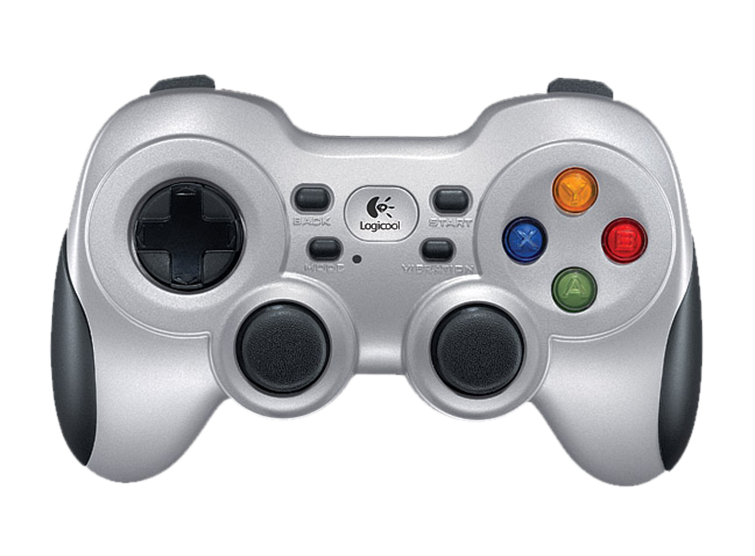
\includegraphics[width=65truemm, clip]{images/f710_overview.png}
    \label{fig:f710_overview}
    \caption{Logicool F710 Gamepad}
  \end{figure}

  有線接続のF310は2310円,無線接続のF710は4950円と安価に入手することができ,ロボットの操縦用コントローラとして使用することもできます.

\subsection{ゲームパッドの入力モード}

  310/F710ゲームパッドは2つの入力モードを持っており,物理スイッチによってモードを切り替えることができます.

  \begin{itemize}
    \item \textsf{DirectInput}モード:他のゲームパッドと同じ挙動を示すモード
    \item \textsf{XInput}モード:Xbox360コントローラをPCに繋いだときと同じ挙動を示すモード
  \end{itemize}

  \noindent
  モード切替スイッチは,F310には本体背面に,F710は本体側面上部に付いています.

  \begin{figure}[ht]
    \centering
    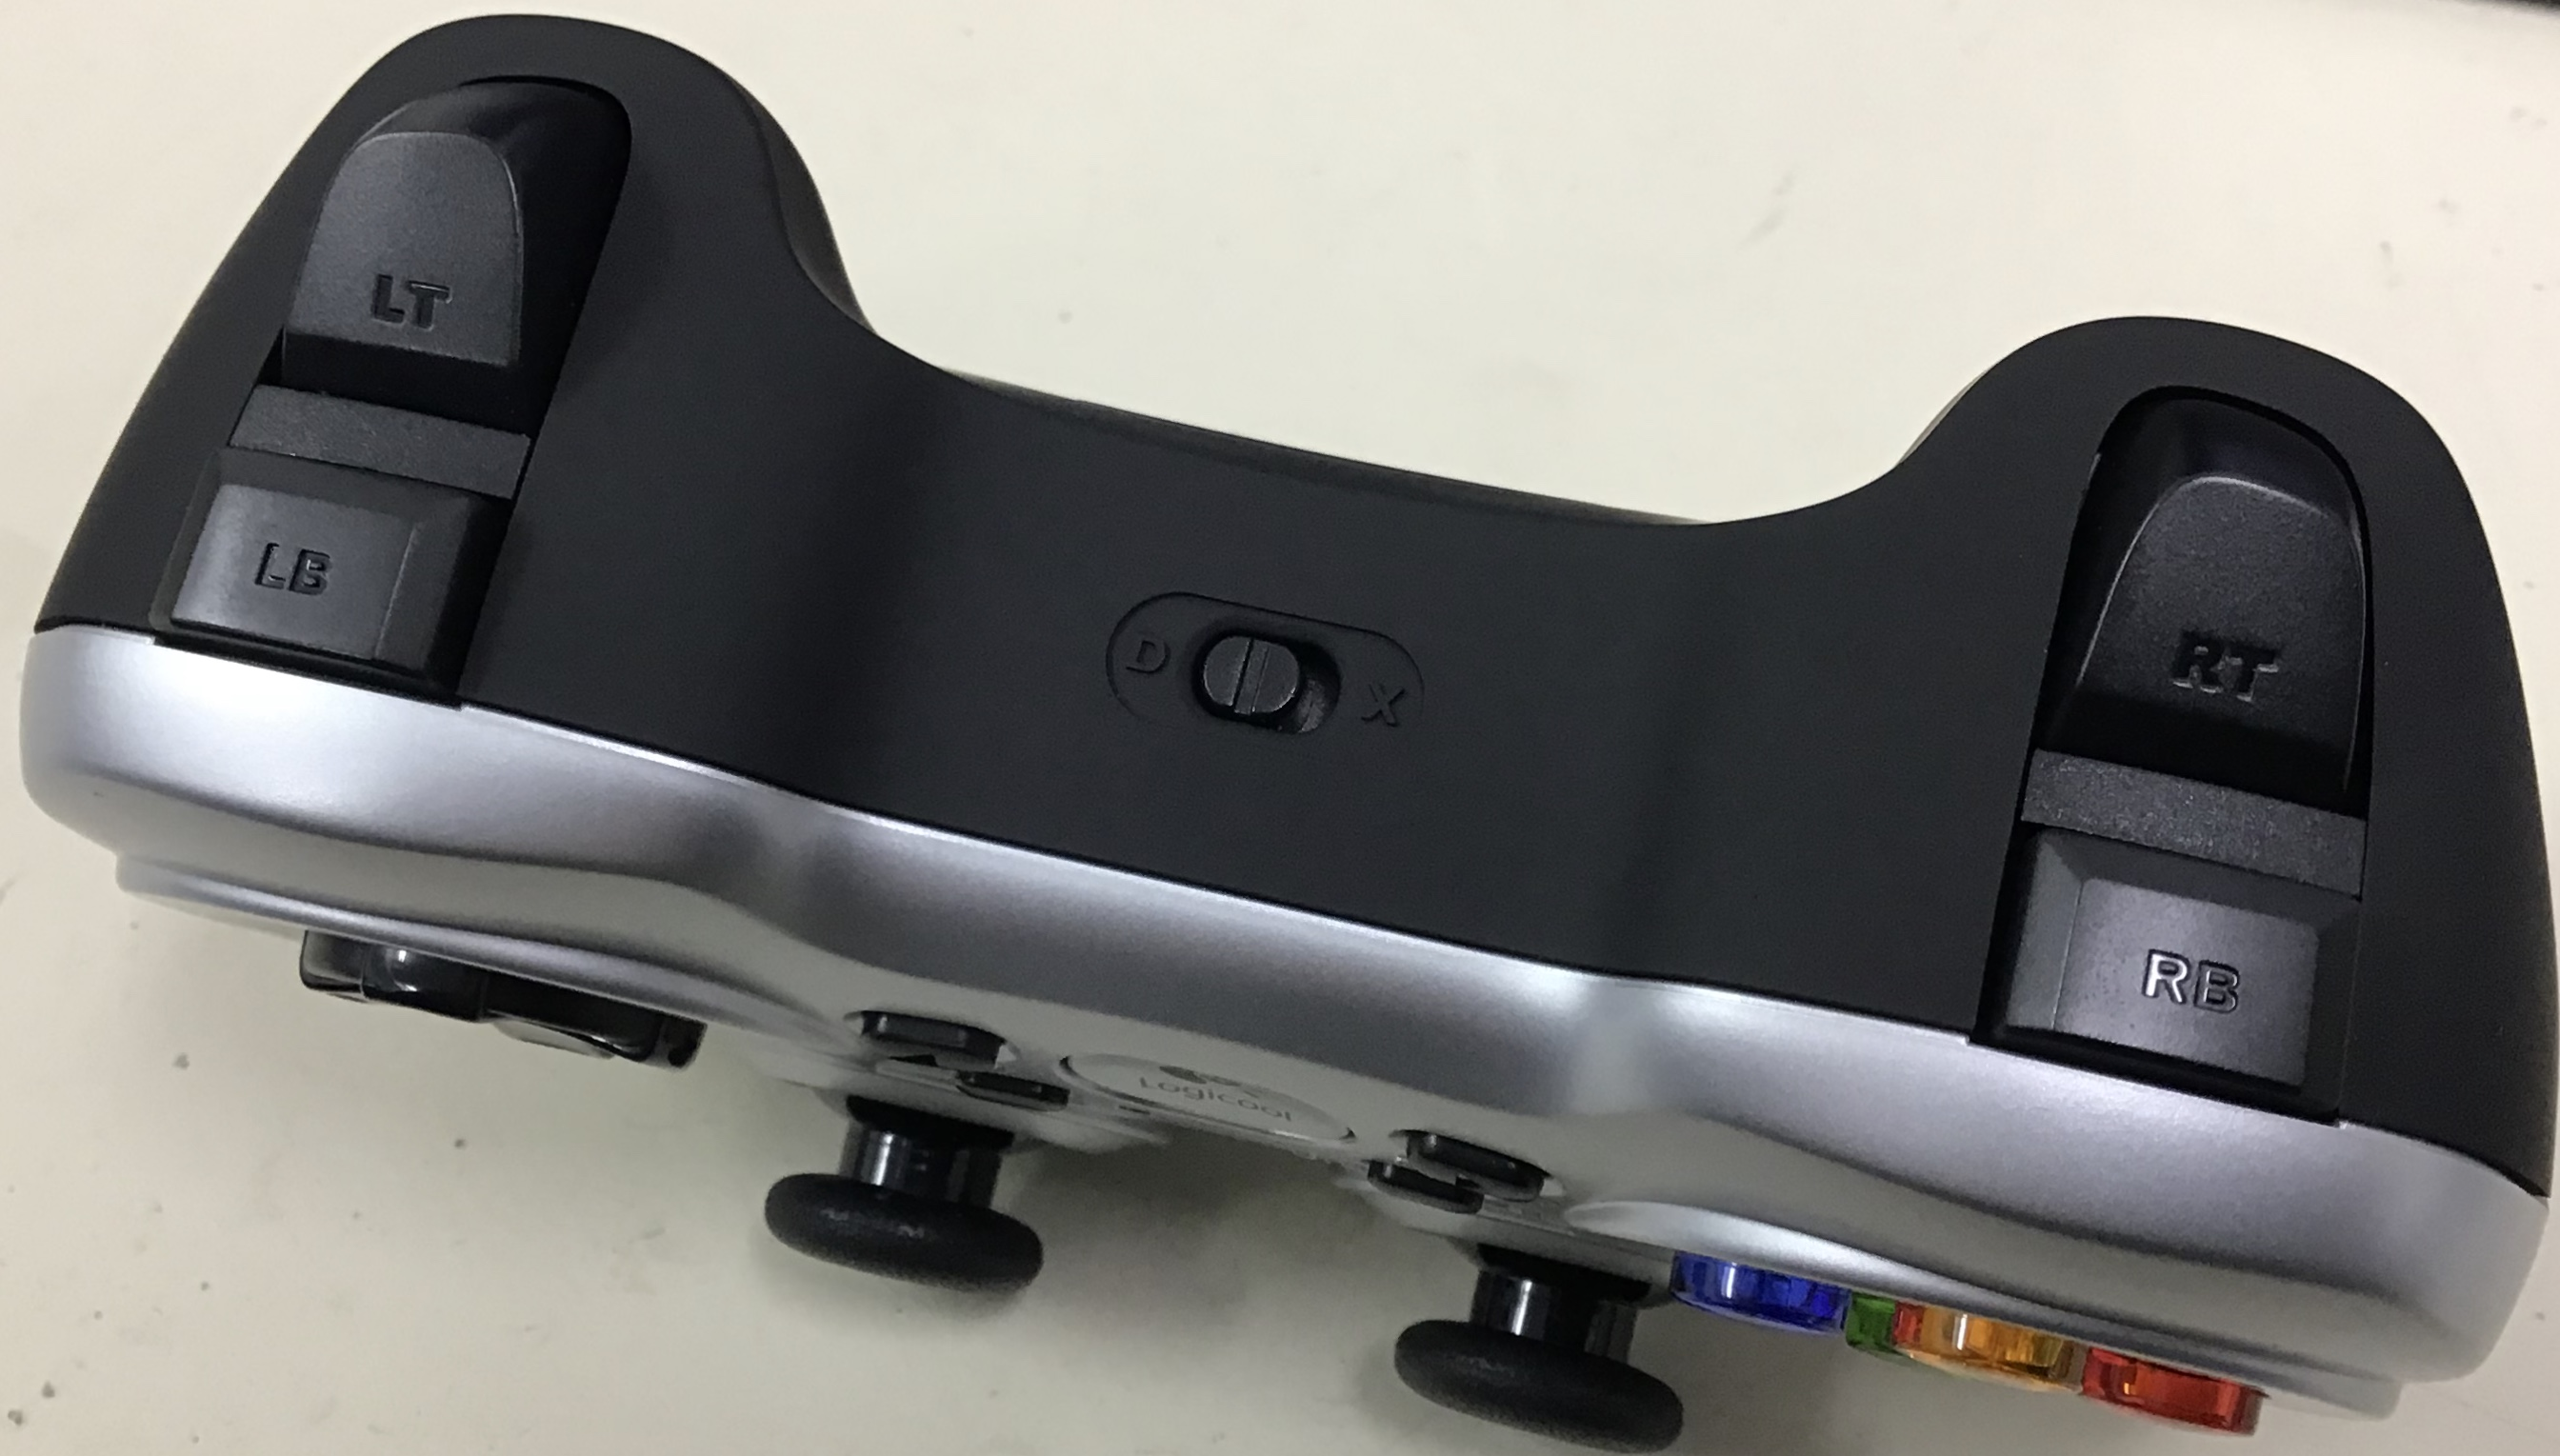
\includegraphics[clip, width=65truemm]{images/mode_switch.jpg}
    \label{fig:mode_switch}
    \caption{Mode Selector Switch for F710}
  \end{figure}

  ROSパッケージの\textsf{joy}\footnote{\url{http://wiki.ros.org/joy}}からF310/F710ゲームパッドを使用するときは,\textsf{DirectInput}モードを使用する必要があります.

\subsection{\textsf{DirectInput}モードのキーマッピング}

\textsf{DirectInput}モードでROSに接続した際のF310/F710ゲームパッドのキーマッピングを表\ref{tab:buttom_mapping}及び表\ref{tab:axis_mapping}に示します.

\textsf{sensor\_msgs/Joy}\footnote{\url{http://docs.ros.org/en/melodic/api/sensor_msgs/html/msg/Joy.html}}型メッセージでは,ゲームパッドの各軸・各ボタンの信号の値が\textsf{axes}と\textsf{buttons}の2つのリストに格納されます.
各リストに対してインデックスを指定することで,対応するボタン・軸のデータを得ることができます.

\begin{table}[h]
  \begin{center}
    \caption{Button Mapping of F310/F710 Gamepad in ROS}
    \begin{tabular}{|c|c|c|c|c|c|c|c|c|c|c|c|c|} \hline
      Buttons & X & A & B & Y & LB & RB & LT & RT & BACK & START & LeftStick & RightStick \\ \hline
       index  & 0 & 1 & 2 & 3 & 4  & 5  & 6  & 7  & 8    &   9   &   10      &     11     \\ \hline
    \end{tabular}
    \label{tab:buttom_mapping}
  \end{center}
\end{table}

\begin{table}[h]
  \begin{center}
    \caption{Axis Mapping of F310/F710 Gamepad in ROS}
    \begin{tabular}{|c|c|c|c|c|c|c|c|c|c|c|c|c|} \hline
      Axis  & Left Horiz. & Left Vert. & Right Horiz. & Right Vert. & Arrow Horiz. & Arrow Vert. \\ \hline
      index & 0 & 1 & 2 & 3 & 4  & 5 \\ \hline
    \end{tabular}
    \label{tab:axis_mapping}
  \end{center}
\end{table}

\subsection{ゲームパッド起動用ファイルを準備する}

F310/F710ゲームパッドをROSに接続して,ゲームパッドからロボットへ速度指令を出せるようにしてみましょう.
ゲームパッドから速度指令を出せるようにするには,以下の2つのパッケージに含まれるノードが必要になります.

\begin{itemize}
  \item \textsf{joy}
  \item \textsf{teleop\_twist\_joy}
\end{itemize}

\textsf{joy}パッケージは汎用ゲームパッドのためのROSドライバです.
\textsf{teleop\_twist\_joy}
\footnote{\url{http://wiki.ros.org/teleop_twist_joy}}
は,\textsf{sensor\_msgs/Joy}メッセージを\textsf{geometry\_msgs/Twist}
\footnote{\url{http://docs.ros.org/en/melodic/api/geometry_msgs/html/msg/Twist.html}}
メッセージに変換するためのパッケージです.
\textsf{Twist}型メッセージで速度指令を受け取るタイプのロボットをゲームパッドから動かす際によく使われているパッケージで,ADAMR2でもこのパッケージを使用しています.

この2つのパッケージのノードを同時に起動するlaunchファイルを\textsf{joy.launch}とし,\textsf{adamr2\_bringup}というパッケージに保存することにします.
\textsf{teleop\_twist\_joy}パッケージを利用するには適切なコンフィグファイルが必要となりますが,それも\textsf{adamr2\_bringup}パッケージに置いておくことにします.

まずはパッケージを作ります.
コード\ref{code:create_adamr2_bringup}のコマンドを実行して,ROSワークスペースに\textsf{adamr2\_bringup}パッケージを作ります.

\begin{lstlisting}[language=sh, label=code:create_adamr2_bringup, caption=Create \textsf{adamr2\_bringup} Package]
cd ~/catkin_ws/src
catkin create pkg adamr2_bringup
\end{lstlisting}

\textsf{adamr2\_bringup}パッケージの中には2つのディレクトリを作ります.
\textsf{launch/}ディレクトリと\textsf{config/}ディレクトリです.
まずはlaunchファイルを準備します.\textsf{launch/}ディレクトリを作成し,\textsf{joy.launch}という名前のlaunchファイルを作成します.
そして,コード\ref{code:joy_launch}のような内容を記述します.

\begin{lstlisting}[language=XML, label=code:joy_launch, caption=\textsf{joy.launch}]
<launch>
  <arg name="joy_dev" default="/dev/input/js0"/>
  <arg name="config_file_path"
       default="$(find adamr2_bringup)/config/f310.config.yml"/>

  <group ns="/adamr2/diff_drive_controller">
    <!-- joy node -->
    <node pkg="joy" type="joy_node" name="joy_node">
      <param name="dev" value="$(arg joy_dev)"/>
      <param name="deadzone" value="0.3" />
      <param name="autorepeat_rate" value="20"/>
    </node>

    <!-- teleop_twist_joy node -->
    <node pkg="teleop_twist_joy" name="teleop_twist_joy" type="teleop_node">
      <rosparam command="load" file="$(arg config_file_path)"/>
    </node>
  </group>
</launch>
\end{lstlisting}

launchファイルのパラメータとして,\textsf{joy\_dev}と\textsf{config\_file\_path}を宣言しています.
\textsf{joy\_dev}はゲームパッドのデバイスファイル名で,ゲームパッドデバイスを1つしか接続していない場合は\textsf{/dev/input/js0}になります.
\textsf{config\_file\_path}は\textsf{teleop\_twist\_joy}パッケージのノードに与えるパラメータを記述したコンフィグファイルのパスです.
まだ作成していないので,このままではlaunchファイルを実行することはできません.

このlaunchファイルでは,\textsf{\<group ns\>}タグで名前空間を設定しています.
\textsf{joy\_node}と\textsf{teleop\_node}は名前空間\textsf{/adamr2/diff\_drive\_controller}の下に置かれ,トピックやパラメータの名前が変化します.
名前空間の設定を行う理由は,対向2輪ロボット用のコントローラである\textsf{diff\_drive\_controller}が,名前空間の下に置かれた速度指令トピックを受信するようになっているためです.

次に,\textsf{teleop\_node}のためのコンフィグファイルを記述します.
ROSでは,ノードに与えるパラメータを1つのファイルにまとめて記述する際に,YAML形式のファイルを使用します.
\textsf{adamr2\_bringup}パッケージディレクトリ直下に\textsf{config/}ディレクトリを作り,\textsf{f310.config.yml}
\footnote{YAML形式のファイルの拡張子は\textsf{.yaml}と\textsf{.yml}が使え(てしまい)ますが,ロボットのシステムを組む際はどちらかに統一した方が良いです.ここでは\textsf{.yml}で統一していますが,ROSでSLAMをしたときに保存されるマップデータのYAMLファイル拡張子が\textsf{.yaml}なので,\textsf{.yaml}で統一した方が良いのかもしれません.}
という名前のファイルを作成します.
そして,コード\ref{code:f310_config_yml}のような内容を記述します.

\begin{lstlisting}[language=yaml, label=code:f310_config_yml, caption=\textsf{f310.config.yml}]
axis_linear: 1
scale_linear: 0.3
scale_linear_turbo: 0.5

axis_angular: 0
scale_angular: 0.94
scale_angular_turbo: 1.57

enable_button: 1
enable_turbo_button: 2
\end{lstlisting}

この設定では,左アナログスティックの縦軸が直進速度,横軸が旋回速度に対応するようになっています.
また,押しているボタンによって速度のスケールが変わるようになっており,Aボタンは通常のスケール,Bボタンでターボスケールになるようになっています.
スケールの具体的な値は\textsf{scale\_linear}と\textsf{scale\_angular}で指定しています.

より詳細なパラメータの設定方法は,\textsf{teleop\_twist\_joy}のROS Wikiのページを参照してください.

\subsection{ゲームパッドを使ってみる}

launchファイルおよび設定ファイルのの準備が終わったので,実際にゲームパッドをROS上で使ってみます.

PCにゲームパッドを接続し,正しく認識されているかどうかを確認してください.
デバイスファイルが存在するかどうかのチェックは,コード\ref{code:check_gamepad_device_path}のコマンドで行うことができます.

\begin{lstlisting}[language=sh, label=code:check_gamepad_device_path, caption=Check Device File of Gamepad]
ls /dev/input/js*
\end{lstlisting}

「\textsf{/dev/input/js0}」のような表示がターミナルに表示されれば問題ありません.
また,Ubuntuでゲームパッドが正しく使えるかどうかをテストするソフトウェアである「\textsf{jstest-gtk}」があります.
ROSから利用する前に,このソフトウェアでチェックをするとよいでしょう.
\textsf{jstest-gtk}は\textsf{apt}コマンドでインストールすることができます.
インストールした後,ターミナルで「\textsf{jstest-gtk}」と実行すればソフトウェアが起動します.

\begin{lstlisting}[language=sh, caption=Install \textsf{jstest-gtk}]
sudo apt update
sudo apt install jstest-gtk
\end{lstlisting}

ゲームパッドのチェックが終わったら,ROSからゲームパッドを利用してみましょう.
パッケージをビルドして環境変数を読み込んだら,launchファイルを実行してみます.

\begin{lstlisting}[language=sh, caption=launch \textsf{joy.launch}]
cd ~/catkin_ws
catkin build
source /opt/ros/melodic/setup.bash
source ~/catkin_ws/devel/setup.bash
roslaunch adamr2_bringup joy.launch
\end{lstlisting}

launchファイルが正しく実行された場合,2つのノードが起動し,\textsf{/adamr2/diff\_drive\_controller/joy}トピックや\textsf{/adamr2/diff\_drive\_controller/cmd\_vel}トピックなどの配信が開始されるはずです.

\end{document}